\documentclass[10pt,a4j,dvipdfmx]{jarticle}
%---------------------------------------------------
\usepackage{hyperref}
\usepackage{pxjahyper}
\usepackage{bm}
\usepackage{graphicx}
\usepackage{amssymb,amsmath}
\usepackage{ascmac}
\usepackage{float}
\usepackage{setspace}
\usepackage[dvips,usenames]{color}
\usepackage{colortbl}
\usepackage{algorithm}
\usepackage{algorithmic}
\usepackage{setspace}
\usepackage{subfigure}
\usepackage{here}
\usepackage[deluxe,bold]{otf}
\usepackage[haranoaji]{pxchfon}
\usepackage{redeffont}
\usepackage{listings,jlisting} %日本語のコメントアウトをする場合jvlisting(もしくはjlisting)が必要
\usepackage{booktabs}
\usepackage{siunitx}
\usepackage{fancybox}
%---------------------------------------------------
% \definecolor{bl}{rgb}{0.94,0.97,1}
% \definecolor{gr}{rgb}{0.5,0.5,0.5}
% \makeatletter
% \def\section{\newpage\@startsection {section}{1}{\z@}{2.3ex plus -1ex minus -.2ex}{2.3 ex plus .2ex}{\Large\bfseries}}
% \makeatother
%---------------------------------------------------
\setlength{\textwidth}{160truemm}
\setlength{\textheight}{240truemm}
\setlength{\topmargin}{-14.5truemm}
\setlength{\oddsidemargin}{-0.5truemm}
\setlength{\headheight}{0truemm}
\setlength{\parindent}{1zw}
\setlength{\abovedisplayskip}{-2pt} % 数式上部のマージン
\setlength{\belowdisplayskip}{-2pt} % 数式下部のマージン
%---------------------------------------------------
\setstretch{1.2}
%---------------------------------------------------
\renewcommand{\subfigtopskip}{5pt}	% 図の上の隙間。上図の副題と下図の間。
\renewcommand{\subfigbottomskip}{0pt} % 図の下の隙間。副題と本題の間。
\renewcommand{\subfigcapskip}{-6pt}	% 図と副題の間
\renewcommand{\subcapsize}{\scriptsize} % 副題の文字の大きさ
\newcommand{\mysection}[1]{\newpage\vspace{-20pt}\section{#1}}
\newcommand{\mysubsection}[1]{\vspace{-20pt}\subsection{#1}}
\newcommand{\mysubsubsection}[1]{\vspace{-10pt}\subsubsection{#1}}
\renewcommand{\lstlistingname}{ソースコード}
\newcommand{\tsuyo}[1]{\textbf{\textgt{#1}}}
%---------------------------------------------------
% ヘッダーとフッターの設定
\usepackage{fancyhdr}
\rhead{ME2208\CID{8705}橋尚太郎}
\chead{}
\lhead{計算力学 課題2}
\cfoot{\thepage}

\rfoot{}
\begin{document}
%---------------------------------------------------
\setlength{\abovedisplayskip}{1.5pt} 
\setlength{\belowdisplayskip}{0pt}
%---------------------------------------------------
%ここからソースコードの表示に関する設定
\lstset{
  language={C++},
  basicstyle={\ttfamily},
  identifierstyle={\small},
  commentstyle={\ttfamily\color[rgb]{0,0.5,0}},
  keywordstyle={\small\bfseries\color[rgb]{0,0,1}},
  ndkeywordstyle={\small},
  stringstyle={\small\ttfamily},
  frame=tRBl,
  breaklines=true,
  columns=[l]{fullflexible},
  numbers=left,
  xrightmargin=0zw,
  xleftmargin=3zw,
  numberstyle={\scriptsize},
  stepnumber=1,
  numbersep=1zw,
  lineskip=-0.5ex,
  morecomment=[l]{//}
}
%ここまでソースコードの表示に関する設定
%---------------------------------------------------

\pagenumbering{arabic}
\pagestyle{fancy}
\setlength{\headheight}{5truemm}

\mysection{目的}
第5章の内燃機関の性能評価に関する項目を実際に実験して確かめる。
\mysection{原理}
\subsection{空気理論サイクル}
ガソリンエンジンに代表される火花点火式のピストンエンジンサイクルは\tsuyo{オットーサイクル(Otto cycle)}と呼ばれ、
その$p$-$V$線図は図\ref{im1}に示される。
4サイクルエンジンの場合、図\ref{im1}の過程$0 \rightarrow 1$において、ガスの吸気が行われ、($P_1, T_1$)がガスの初期状態となる。
過程$1 \rightarrow 2$において、断熱圧縮を行い、過程$2 \rightarrow 3$において爆発的な燃焼が行われ、系は熱源から$Q_1$の熱量を受け取り、
最高圧力、最高温度 ($P_3, T_3$)となる。過程$3 \rightarrow 4$において、断熱膨張が行われ、外部に対して仕事を行う。
過程$4 \rightarrow 1$で放熱し、その後の状態は$(P_1, T_4)$となる。過程$1 \rightarrow 0$でガスの排気を行い、過程$0 \rightarrow 1$の吸入過程と
打ち消し合う。過程$2 \rightarrow 3$のように、容積一定のもとで加熱が行われるので、オットーサイクルは\tsuyo{等容サイクル(constant volume cycle)}とも呼ばれる。\cite{netsu}
\begin{figure}[h]
  \begin{center}
  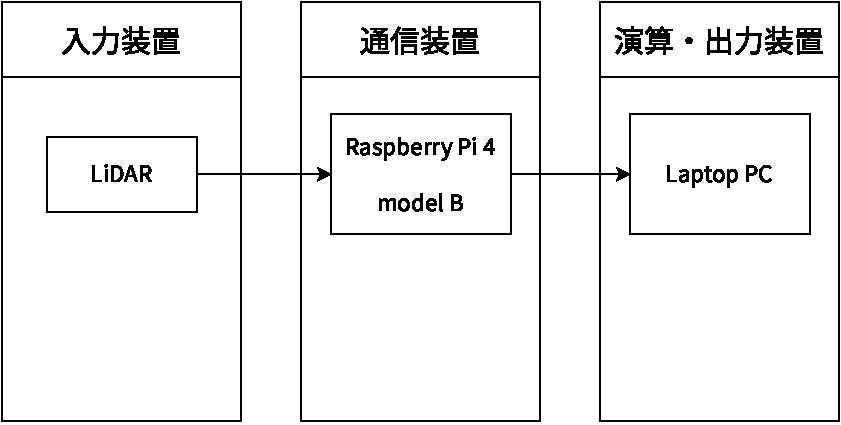
\includegraphics[width=.8\columnwidth]{img/1.pdf}
  \caption{オットーサイクルの$p$-$v$線図\cite{shiryo}}
  \label{im1}
  \end{center}
\end{figure}
以上のように、空気理論サイクルでは2つの断熱変化と2つの等容変化で構成されており、このサイクルの\tsuyo{理論熱効率(theoretical thermal efficiency)}を$\eta_{th}$とすると次式で表される。
$$\eta_{th} = \frac{Q_1-Q_2}{Q_1}\times 100 = 1-\frac{Q_2}{Q_1} \times 100 = 1-\frac{T_4-T_1}{T_3-T_2} \times 100 = 1-\frac{1}{\varepsilon^{\kappa-1}} \times 100 \si{[\%]}$$

\mysubsection{エンジン性能指標と熱勘定}
\begin{description}
  \setlength{\parskip}{0cm} % 段落間
  \setlength{\itemsep}{0cm} % 項目間
  \item[軸トルク] 回転する軸が出力できる力のこと。単位は\si{[\newton\meter]}。
  \item[軸出力] エンジンの動力取り出し軸における出力のこと。単位は\si{[\kW]}。
  \item[燃料消費率] エンジンの軸出力1\si{[\kW]}あたり1\si{[\hour]}ごとに消費される燃料の質量\si{[\g]}のこと。単
  位は\si{[\g/\kWh]}。
  \item[正味熱効率] 燃料の発熱量に対する軸出力の割合のこと。単位は\si{[\%]}。
  \item[熱勘定] 熱機関の入熱と出熱との熱平衡精算の結果である熱収支を表す方法として、
  燃料の完全燃焼により発生する熱量を100\si{\%}とし、転換したエネルギーが各部にどのように分配されているかを表すこと。
  図示仕事から運動部分の摩擦、補機類の駆動仕事を差引いて実際に機関主軸から取出せる出力を仕事に換算した\tsuyo{正味仕事}、\tsuyo{冷却損失}、\tsuyo{排気損失}および\tsuyo{機械損失}の4項目に分ける。\cite{kanjo}
\end{description}
\mysubsection{特性値の算出}
\tsuyo{特性値で用いる記号}\\
$W$:動力系制動荷重\si{[\newton]}、$N$:動力系回転数\si{[rpm]}、$T_e$:エンジン軸トルク\si{[\newton \meter]}、$P_e$:エンジン軸出力\si{[\kW]}、\\
$b$:測定時間内の燃料消費量\si{[\mL]}、$p_{me}$:正味平均有向圧\si{[\kPa]}、$V_s$:行程容積\si{[\L]}、
$a$:サイクル数/2(4サイクル:$a=2$、2サイクル:$a=1$)、$t$:燃料消費量の測定に要した時間\si{[\sec]}、$\gamma$:燃料密度\si{[0.72 \g/\mL]}、$H_l$:燃料の低位発熱量\si{[46000\kJ/\kg]}、$b_e$:燃料消費率\si{[\g/\kWh]}、$\eta_e$:正味熱効率\si{[\%]}
\begin{description}
  \setlength{\parskip}{0cm} % 段落間
  \setlength{\itemsep}{0cm} % 項目間
  \item[軸トルク] $$T_e = 0.2865 \cdot W \si{[\newton\meter]}$$
  \item[軸出力] $$P_e = \frac{W\cdot N}{33330} \si{[\kW]}$$
  \item[正味平均有向圧] $$p_{me} = \frac{60\times P_e \cdot a}{V_s\cdot N} \times 1000 \si{[\kPa]}$$
  \item[燃料消費率] $$b_e = \frac{\gamma \cdot (b/t)}{P_e} \times 3600 \si{[\g/\kWh]}$$
  \item[正味熱効率] $$\eta_e = \frac{P_e}{{\gamma\cdot (b/t)}\cdot H_l}\times 100 \si{[\%]}$$
  \item[燃料全熱量] $$Q_f = H_l\frac{\gamma(b/t)}{1000} \si{[\kW]}$$
  \item[排気損失] $$\eta_g = \frac{Q_g}{Q_f} \si{[\%]}$$
  \begin{description}
    \setlength{\parskip}{0cm} % 段落間
    \setlength{\itemsep}{0cm} % 項目間
    \item[排気損失熱量] $$Q_g = G_g c_{pg}(\si{TG1}-\si{TA1}) \si{[\kW]}$$
    \item[排気ガス流量] $$G_g = 0.072\sqrt{p_1-p_2}+\frac{\gamma(b/t)}{1000} \si{[\kg/\s]}$$
    \item[差圧] $$p_1 - p_2 = \si{DPA1} \si{[\kPa]}$$
    \item[排気ガス比熱] $$c_{pg}=1.24 \si{[\kJ/(\kg\K)]}$$
    \item[排気ガス温度] $$\si{TG1} \si{[\degreeCelsius]}$$
    \item[吸入空気温度] $$\si{TA1} \si{[\degreeCelsius]}$$
  \end{description}
  \item[冷却損失] $$\eta_w = \frac{Q_w}{Q_f}\times 100 \si{[\%]}$$
  \begin{description}
    \setlength{\parskip}{0cm} % 段落間
    \setlength{\itemsep}{0cm} % 項目間
    \item[冷却損失熱量] $$Q_w = \frac{\si{FW1}}{3600}c_{pw}(\si{TW2}-\si{TW1}) \si{[\kW]}$$
    \item[冷却水流量] $$\si{FW1} \si{[\litre/\hour]}$$
    \item[水の比熱] $$c_{pw} = 4.2 \si{[\kJ/(\kg\K)]}$$
    \item[冷却水出口温度] $$\si{TW2} \si{[\degreeCelsius]}$$
    \item[冷却水入口温度] $$\si{TW1} \si{[\degreeCelsius]}$$
  \end{description}
  \item[機械損失] $$\eta_m = 100 - (\eta_e + \eta_g + \eta_w) \si{[\%]}$$
\end{description}

\mysection{実験方法}
実験装置は、東京メーター製:内燃機関性能総合試験装置 (GWE-88/150R)であり、以下のように乗用車用エンジンと測定器で構成されている。
\begin{description}
  \setlength{\parskip}{0cm} % 段落間
  \setlength{\itemsep}{0cm} % 項目間
  \item[試験エンジン] 名称:2NZ-FE ガソリンエンジン(トヨタ自動車製)、形式:4サイクル4気筒水冷式\\総排気量:1298\si{[cc]}、圧縮比:10.5、最大軸出力:65\si{[\kW]}(6000\si{[rpm]})、最大軸トルク:121\si{[\newton\meter]}(4000\si{[rpm]}) 
  \item [測定器] 絞り弁開閉度計、動力計(腕長さ\tsuyo{286.5\si{[\milli\meter]}})、回転数計、吸入空気差圧計、燃料消費計、面積流量計、温度指示計
  \item [使用燃料] ガソリン、密度:\tsuyo{0.72\si{[\kg/\l]}}、低位発熱量\tsuyo{46000\si{[\kJ/\kg]}}
\end{description}
\mysubsection{回転数変化試験}
絞り弁開度を20\%に固定し、回転数を1600、3200、4800 \si{[rpm]}とした。指示器の計測値が安定したとき、下記項目について測定した。
\begin{description}
  \item[測定項目] 絞り弁開度、動力計制動荷重、動力計回転数、燃料消費時間、吸入空気差圧、
  吸入空気温度、\\排気ガス温度、冷却水流量、冷却水入口温度、冷却水出口温度 
\end{description}

\mysection{結果}
測定結果を表\ref{tb1}、測定結果のプロットを図\ref{plot1}~\ref{plot3}に示す。
に示す。DPA1の測定値に関して、測定値が1の位から小数第2位まで測定できる装置で、
実際の測定値が0.05、0.16、0.22であったため、小数第1位と小数第2位の数値が有効であるとする。
本実験では有効数字を3桁で示す。
$t$に関して、実際の測定値は、10の位から小数第2位の4桁であった。人間が反応するための時間は、
おおよそ0.2\si{[s]}である。これは測定値の0.5\% ~ 1\% の誤差に相当する。
本実験での計算結果に関する人間の測定による誤差の影響は、有効桁の4桁目に現れるため、
人間による時間測定の誤差は無視できるものとして扱い、本実験の数値で$t$の計算結果は有効数字2~3桁とする。

\vspace{-5truemm}
\begin{table}[h]
\centering
\caption{測定結果}
\scalebox{.8}{
\begin{tabular}[t]{crrrrrrrrrr}
\toprule
&THK\si{[\%]}&$N$\si{[rpm]}&$W$\si{[\newton]}&$t$\si{[\s]}&DPA1\si{[\kPa]}&TA1\si{[\degreeCelsius]}&TG1\si{[\degreeCelsius]}&FW1\si{[\l/\hour]}&TW1\si{[\degreeCelsius]}&TW2\si{[\degreeCelsius]}\\
\midrule
実験1&20&1600&314&53.9&0.05&25.4&674&400&22.3&51.0\\
実験2&20&3200&278&30.4&0.16&26.2&756&740&22.3&48.0\\
実験3&20&4800&200&25.8&0.22&27.6&791&785&21.9&52.0\\
\bottomrule
\label{tb1}
\end{tabular}}
\end{table}%

\vspace{-5truemm}
\begin{figure}[h]
  \begin{center}
  \subfigure[測定結果のプロット1]{
  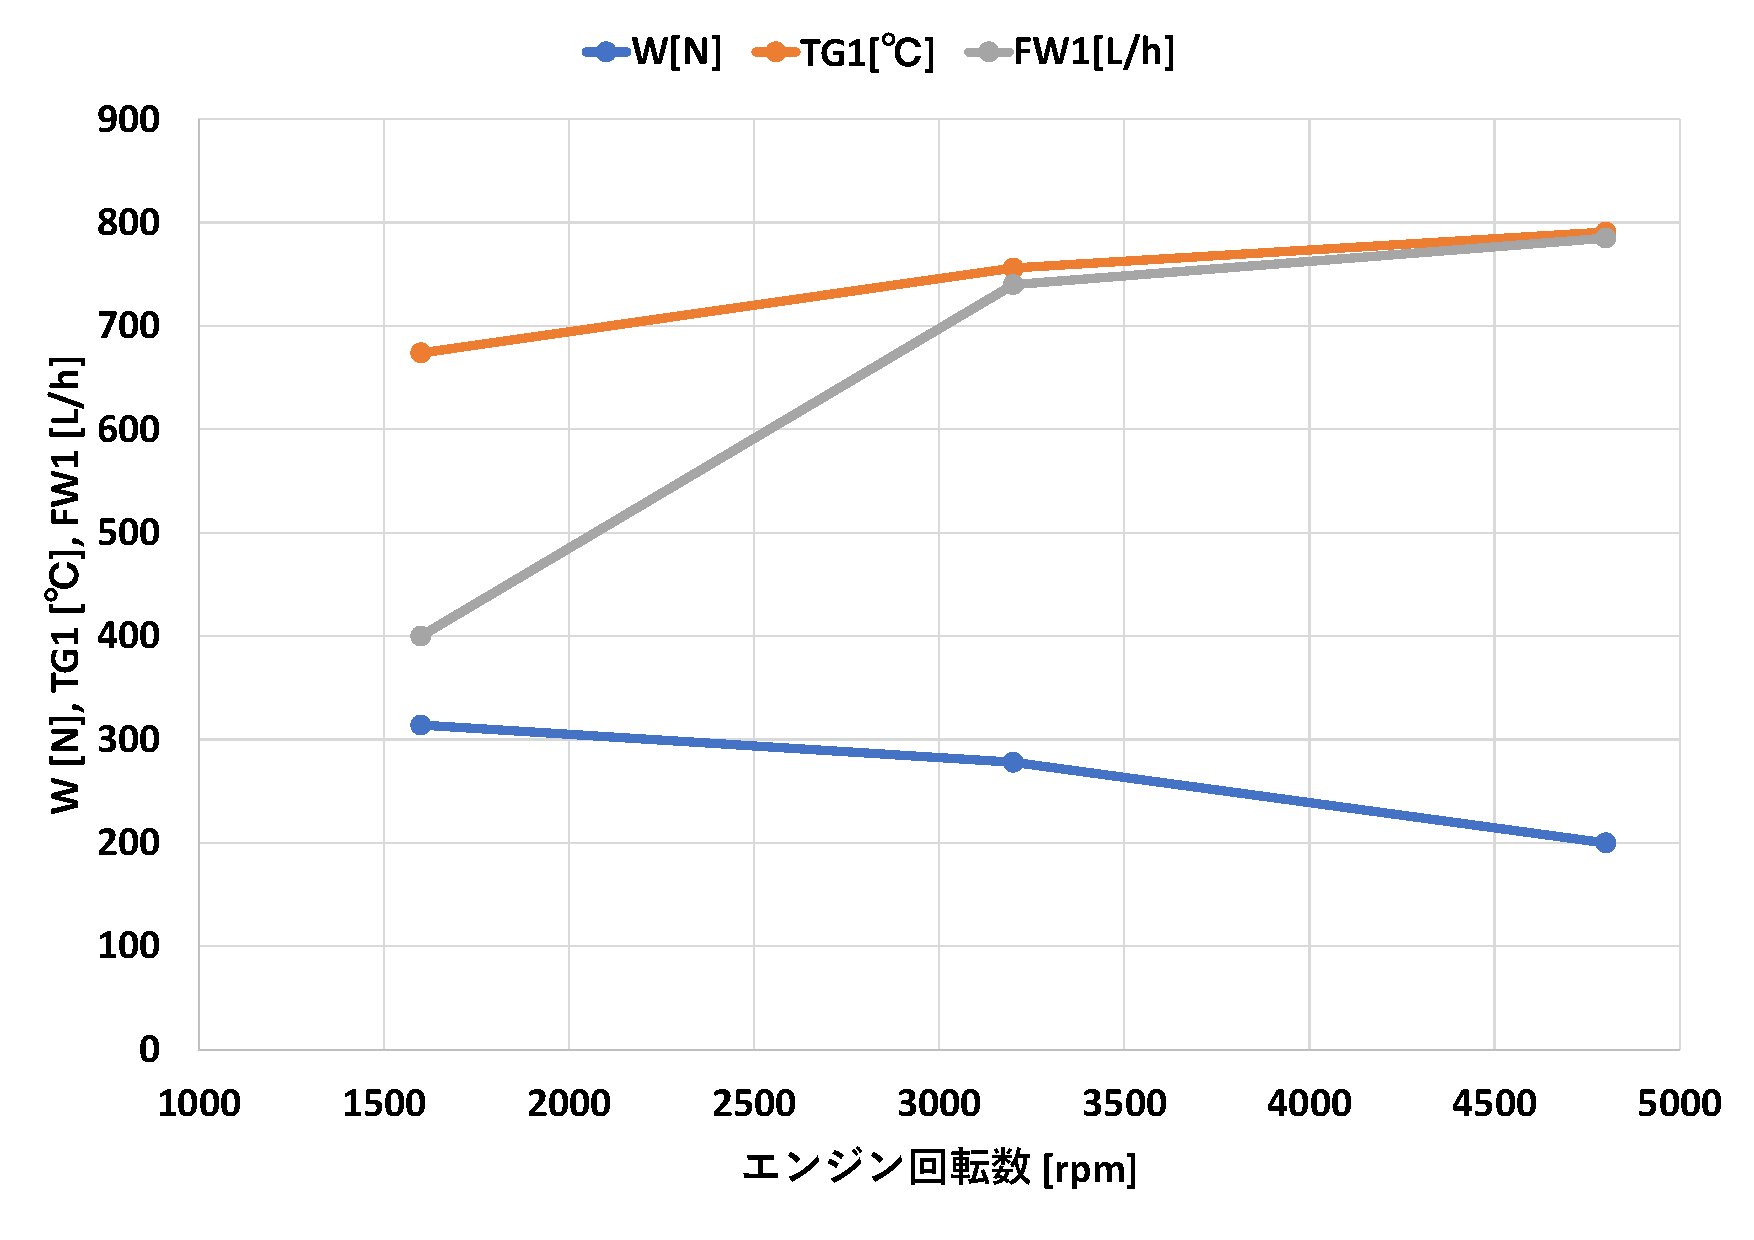
\includegraphics[width=.37\columnwidth]{img/plot1.pdf}
  \label{plot1}
  }
  \subfigure[測定結果のプロット2]{
  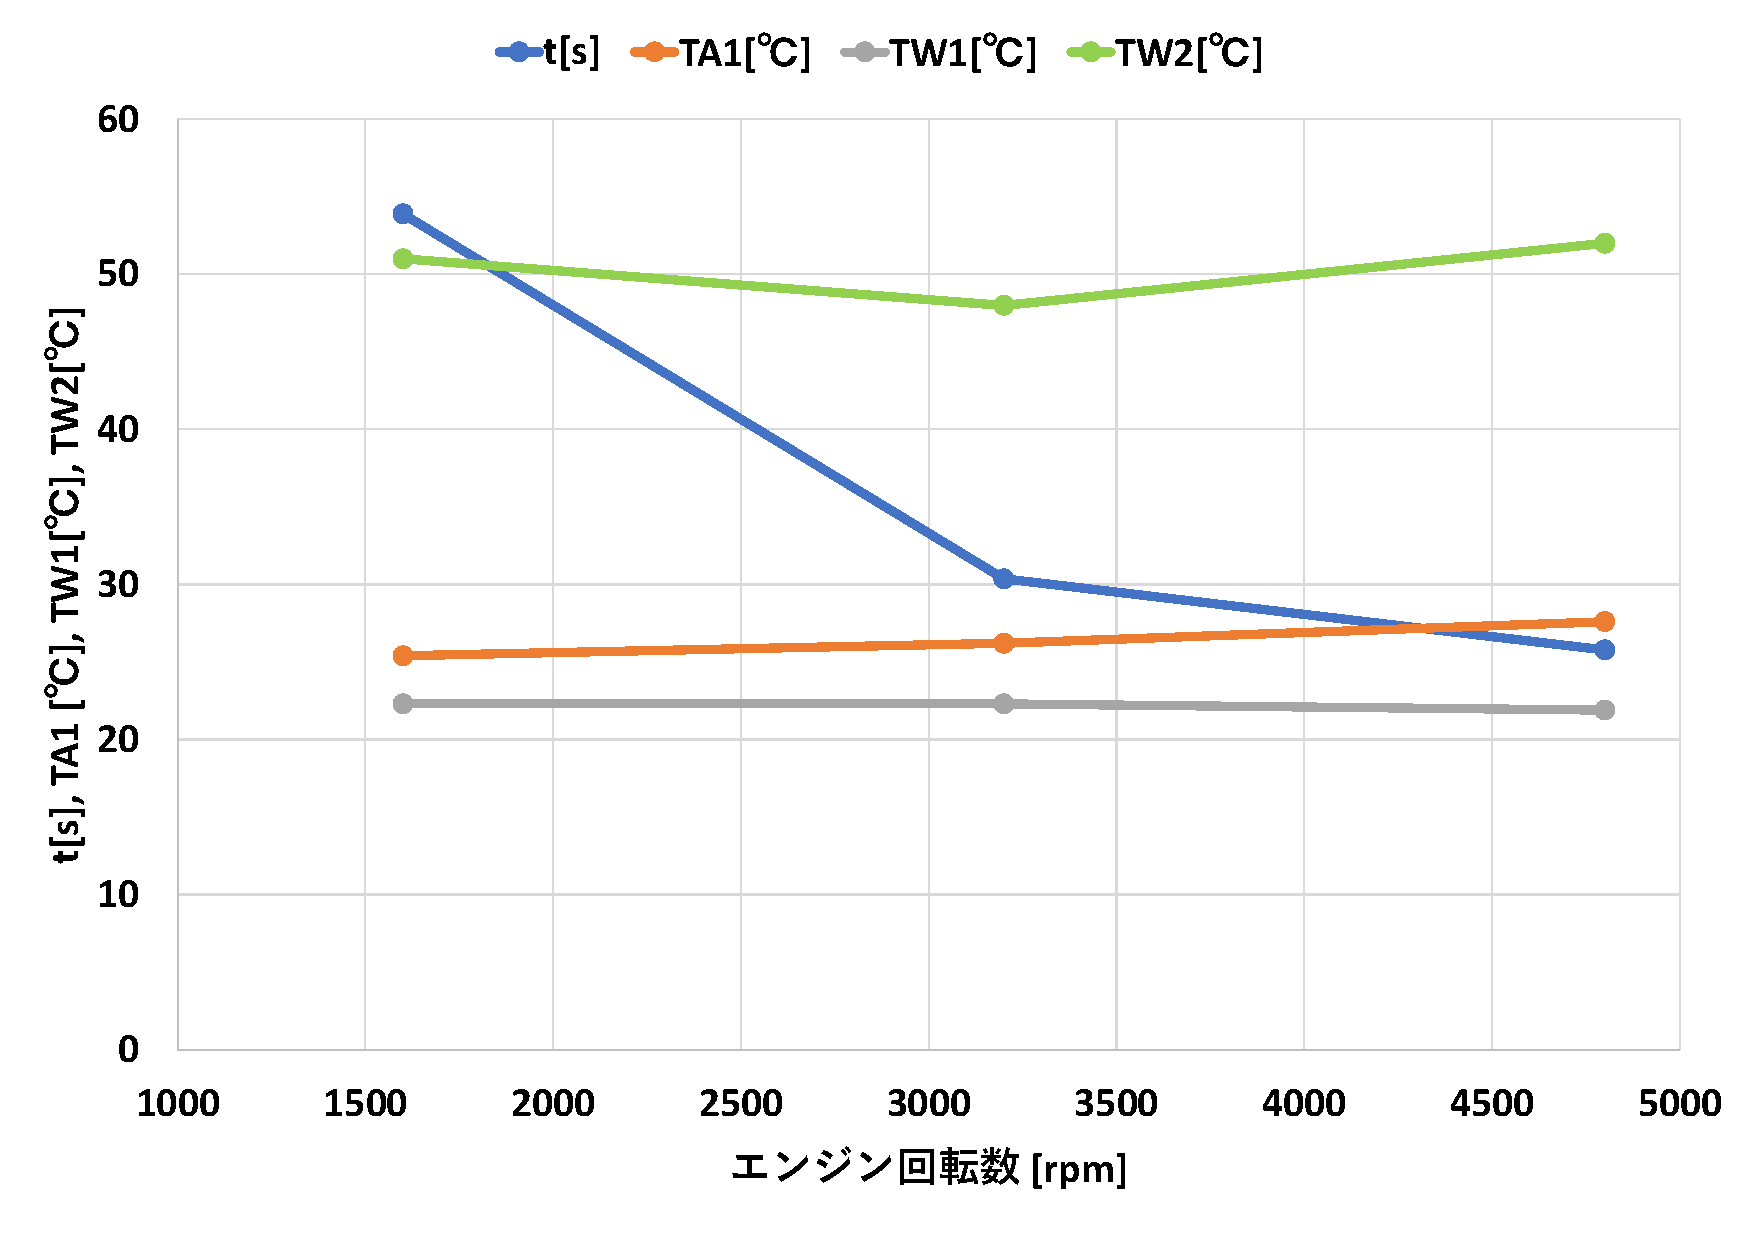
\includegraphics[width=.37\columnwidth]{img/plot2.pdf}
  \label{plot2}
  }
  \subfigure[測定結果のプロット3]{
  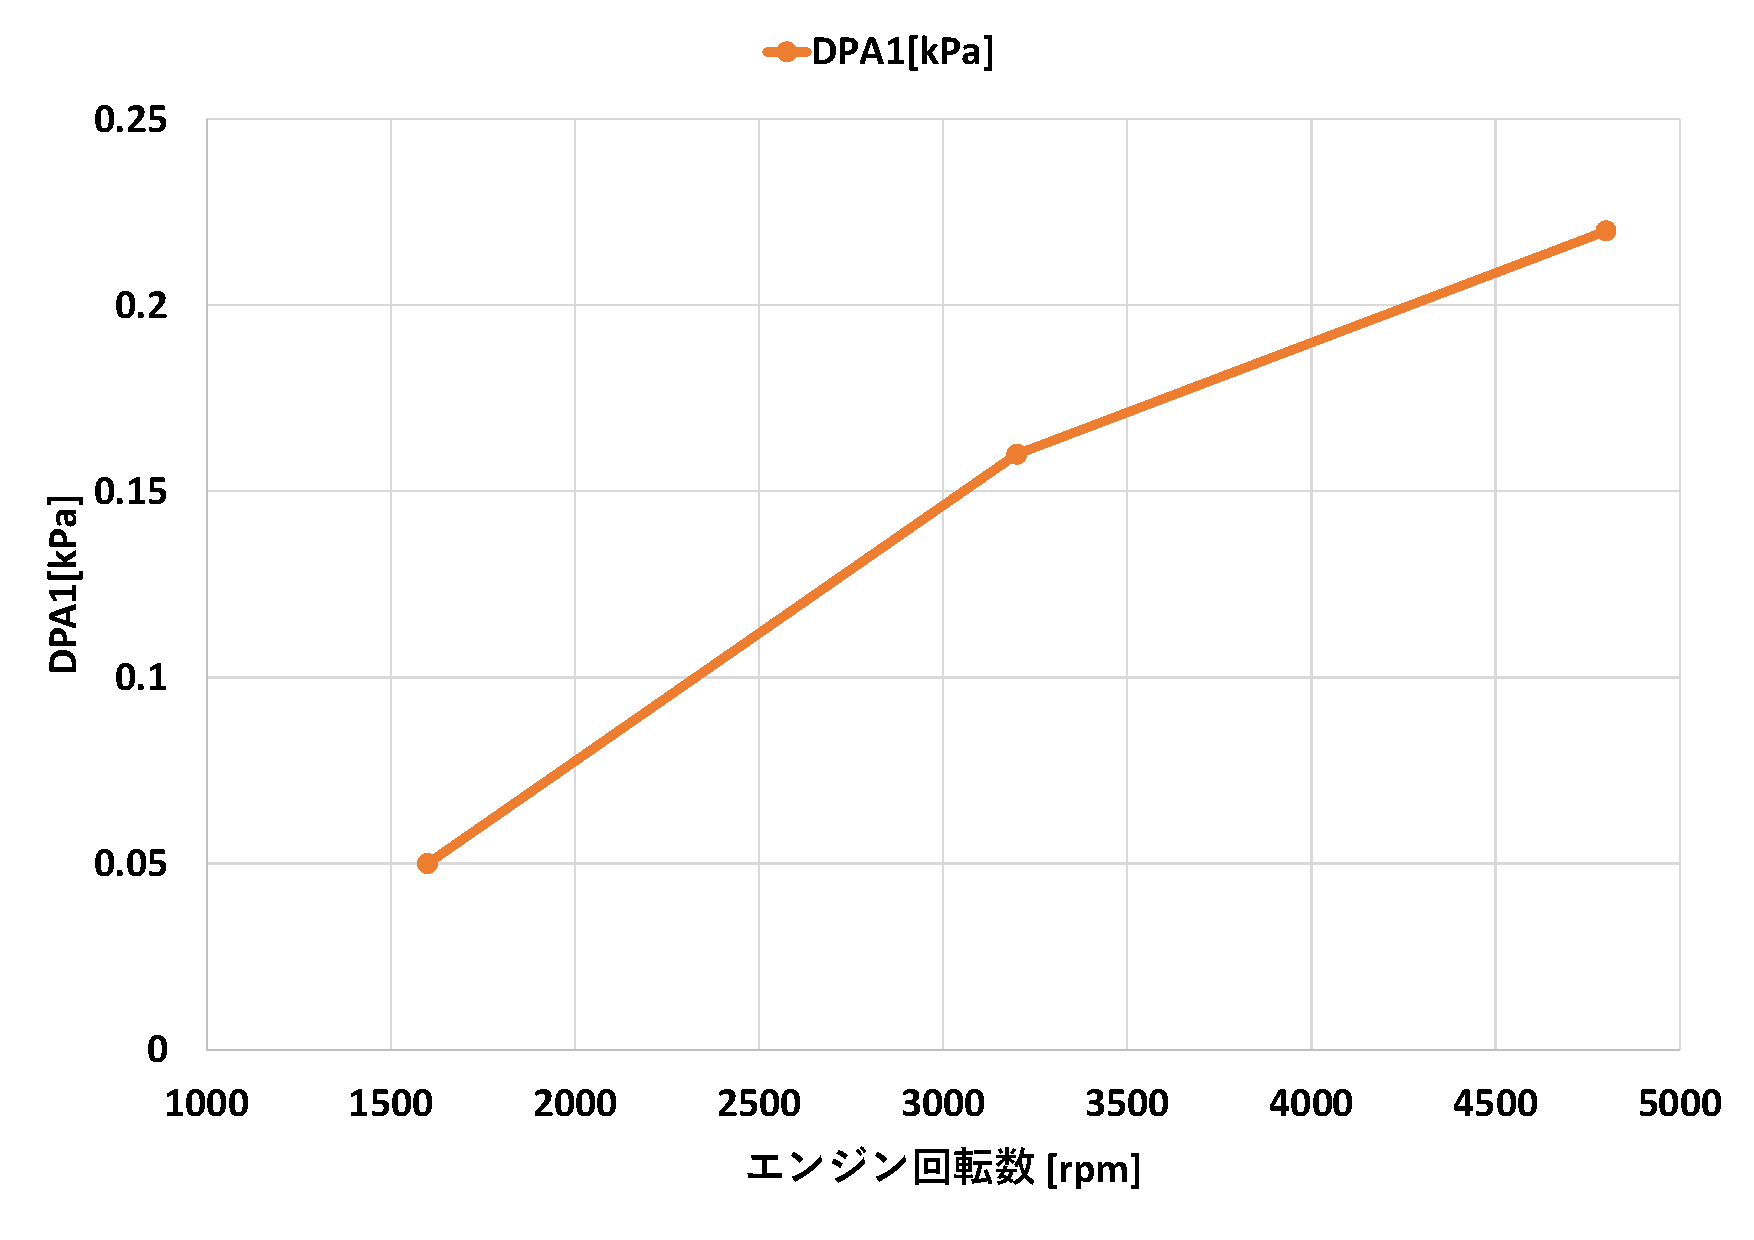
\includegraphics[width=.37\columnwidth]{img/plot3.pdf}
  \label{plot3}
  }
  \caption{測定結果のプロット}
  \end{center}
\end{figure}
\label{plot}

\mysubsection{結果の解析}
測定結果を解析することで得た特性値を表\ref{tb2}に示す。
表中の括弧内の値は図示熱効率に置き換えて算出した値である。
本実験での計算結果の有効数字は、効率は2桁、それ以外は3桁となる。

\begin{table}[h]
  \centering
  \caption{特性値}
  \scalebox{.7}{
  \begin{tabular}[t]{crrrrrrrrrrrr}
  \toprule
  &$N$\si{[rpm]}&$T_e$\si{[\newton\meter]}&$P_e$\si{[\kW]}&$b_e$\si{[\g/\kWh]}&$Q_f$\si{[\kW]}&$\eta_e$\si{[\%]}(※図示熱効率)&$G_g$\si{[\kg/\s]}&$Q_g$\si{[\kW]}&$\eta_g$\si{[\%]}&$Q_w$\si{[\kW]}&$\eta_w$\si{[\%]}&$\eta_m$\si{[\%]}\\
  \midrule
  実験1&1600&90.0&15.1&255&49.2&31 (36)&0.0172&13.8&28&13.4&27&14 (9.2)\\
  実験2&3200&80.0&31.6&256&87.2&31 (36)&0.0307&27.8&31&22.2&25&12 (6.5)\\
  実験3&4800&57.3&28.8&273&103&28 (39)&0.0360&34.1&33&27.6&27&12 (0.75)\\
  \bottomrule
  \label{tb2}
  \end{tabular}}
\end{table}%
$p$-$v$線図を図\ref{pv}、エンジン性能曲線を図\ref{engine}、
熱勘定図を図\ref{shoumi}、図\ref{zushi}に示す。

\begin{figure}[h]
  \begin{center}
  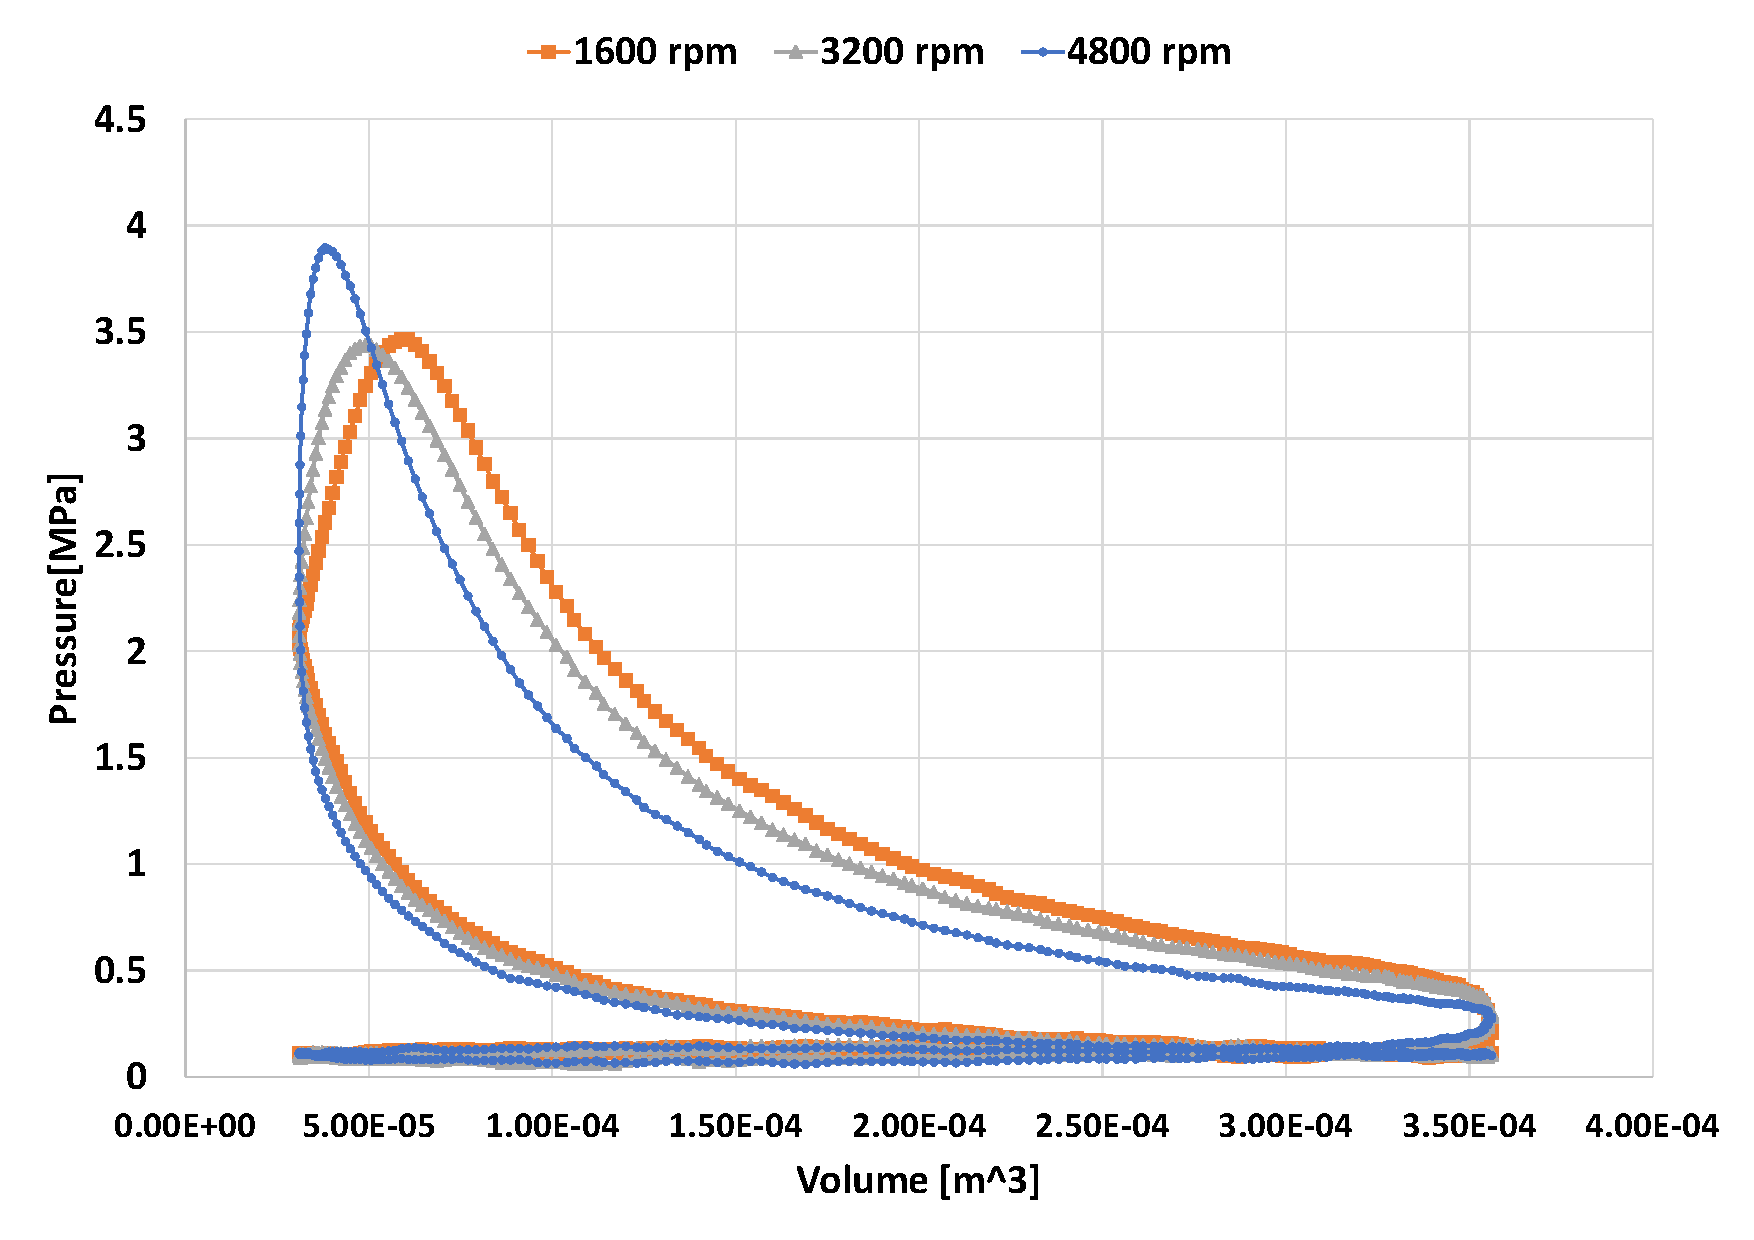
\includegraphics[width=\linewidth]{img/pv_all.pdf}
  \caption{$p$-$v$線図}
  \label{pv}
\end{center}
\end{figure}

\begin{figure}[h]
  \begin{center}
  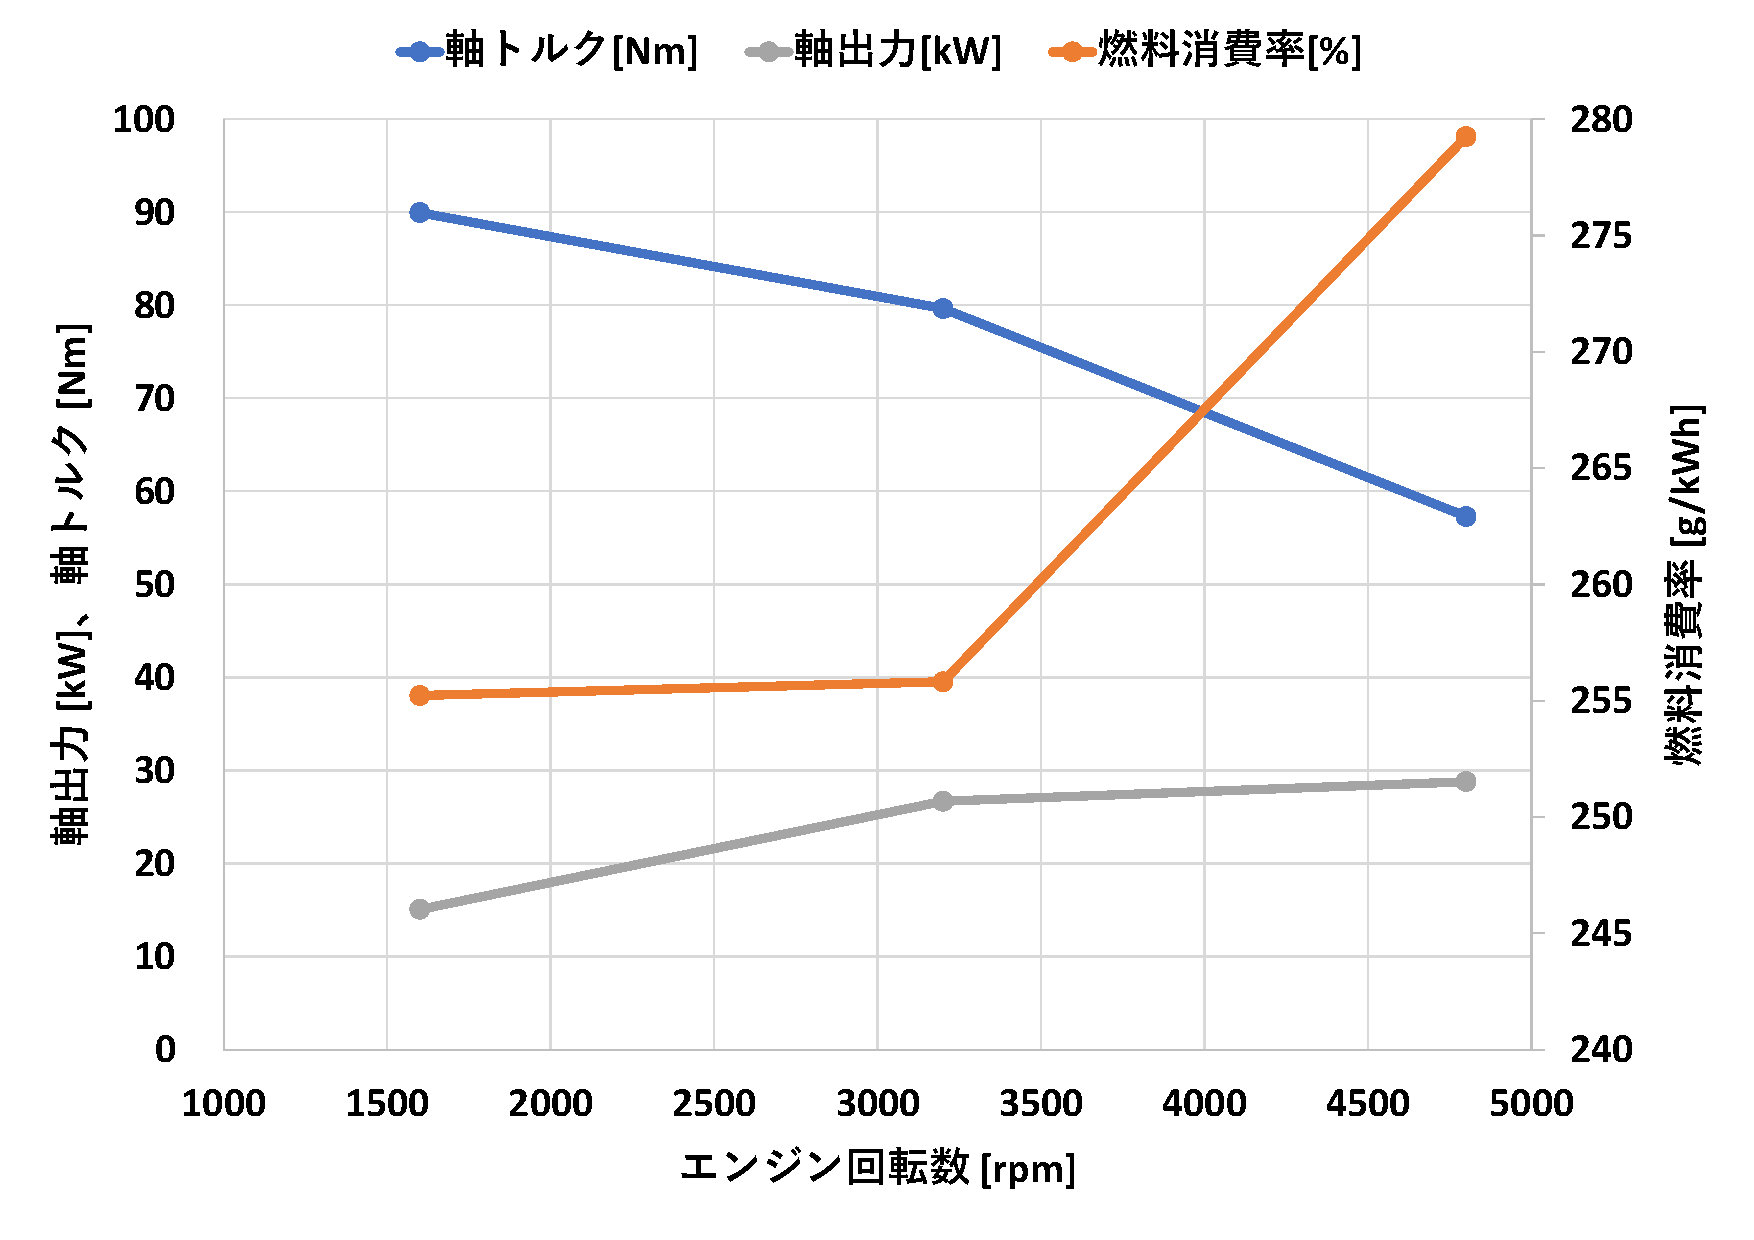
\includegraphics[width=\linewidth]{img/engine_performance.pdf}
  \caption{エンジン性能曲線}
  \label{engine}
  \end{center}
\end{figure}

\begin{figure}[h]
  \begin{center}
  \subfigure[正味熱効率を用いた場合]{
  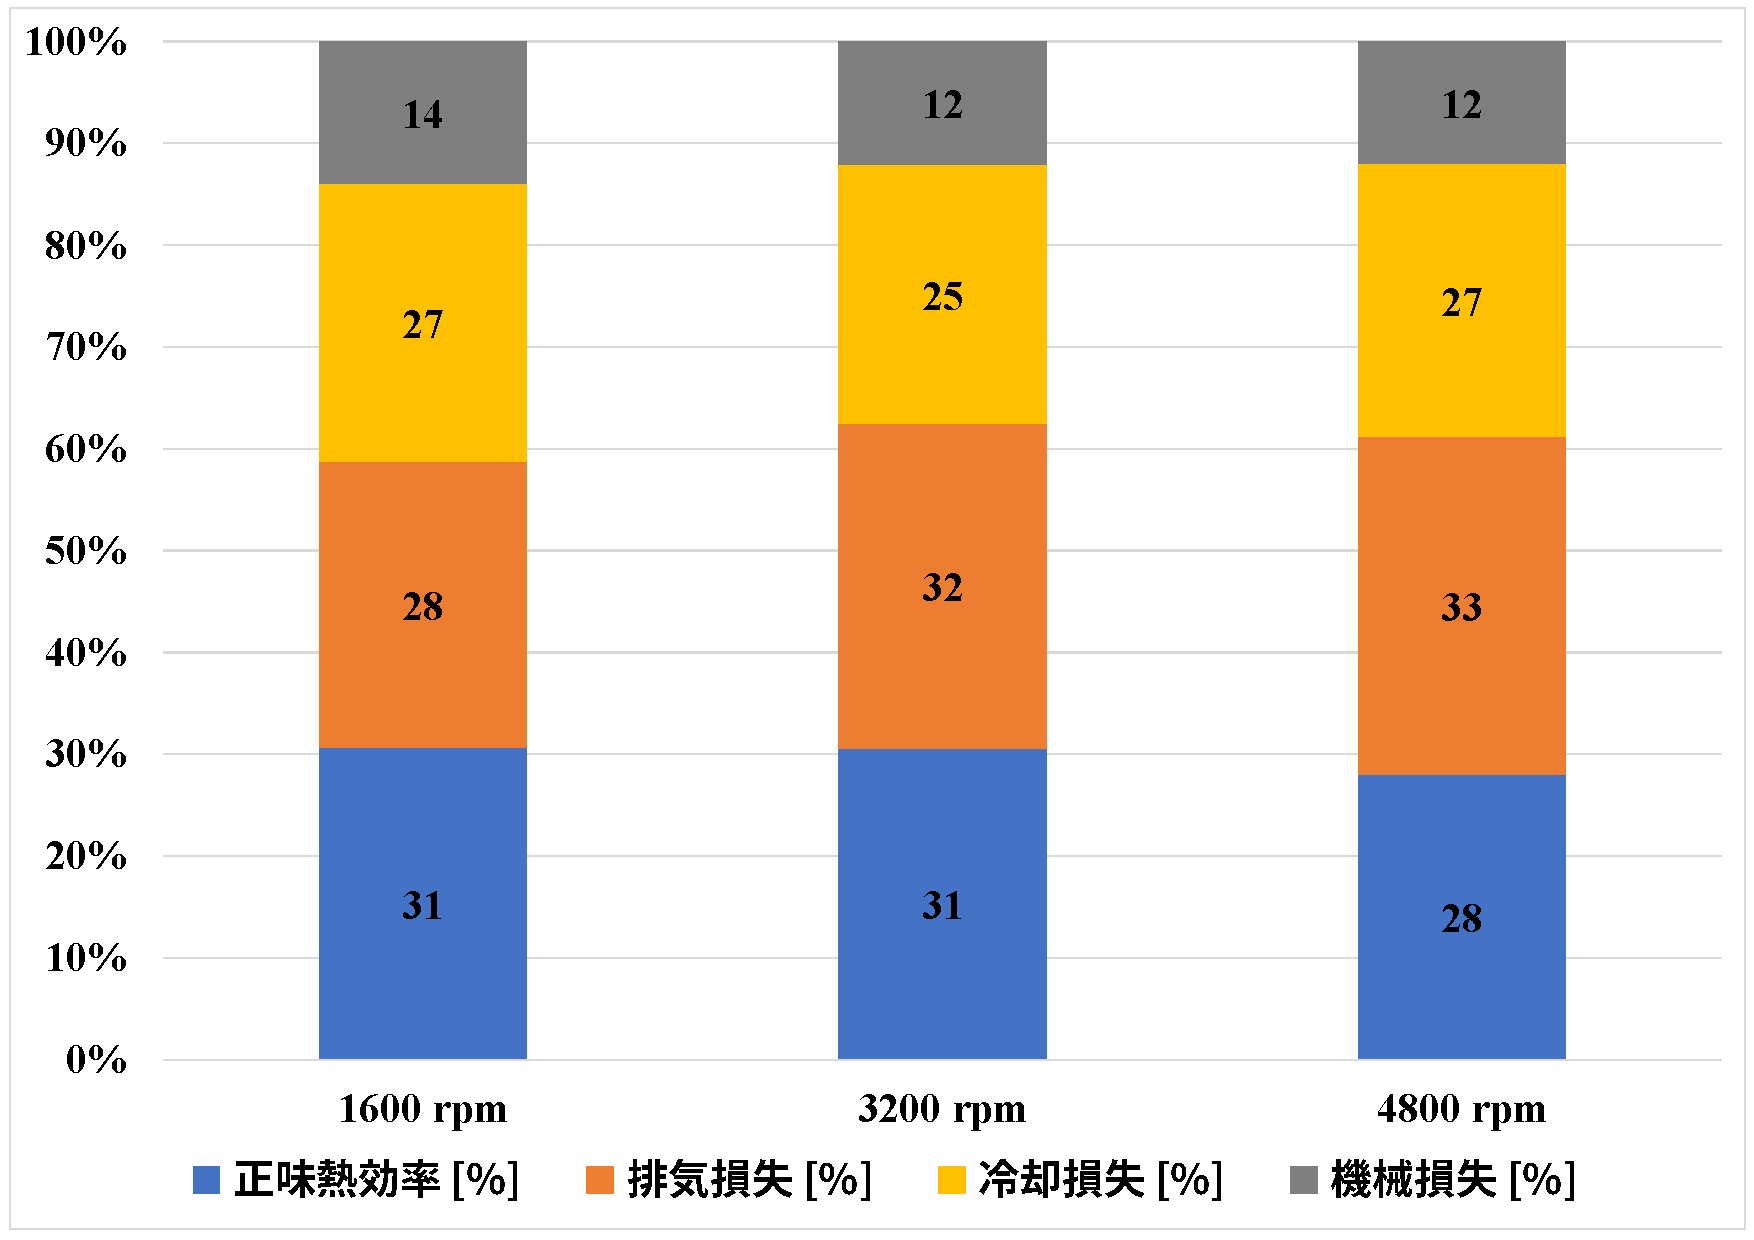
\includegraphics[width=.48\columnwidth]{img/shoumi.pdf}
  \label{shoumi}
  }
  \subfigure[図示熱効率を用いた場合]{
  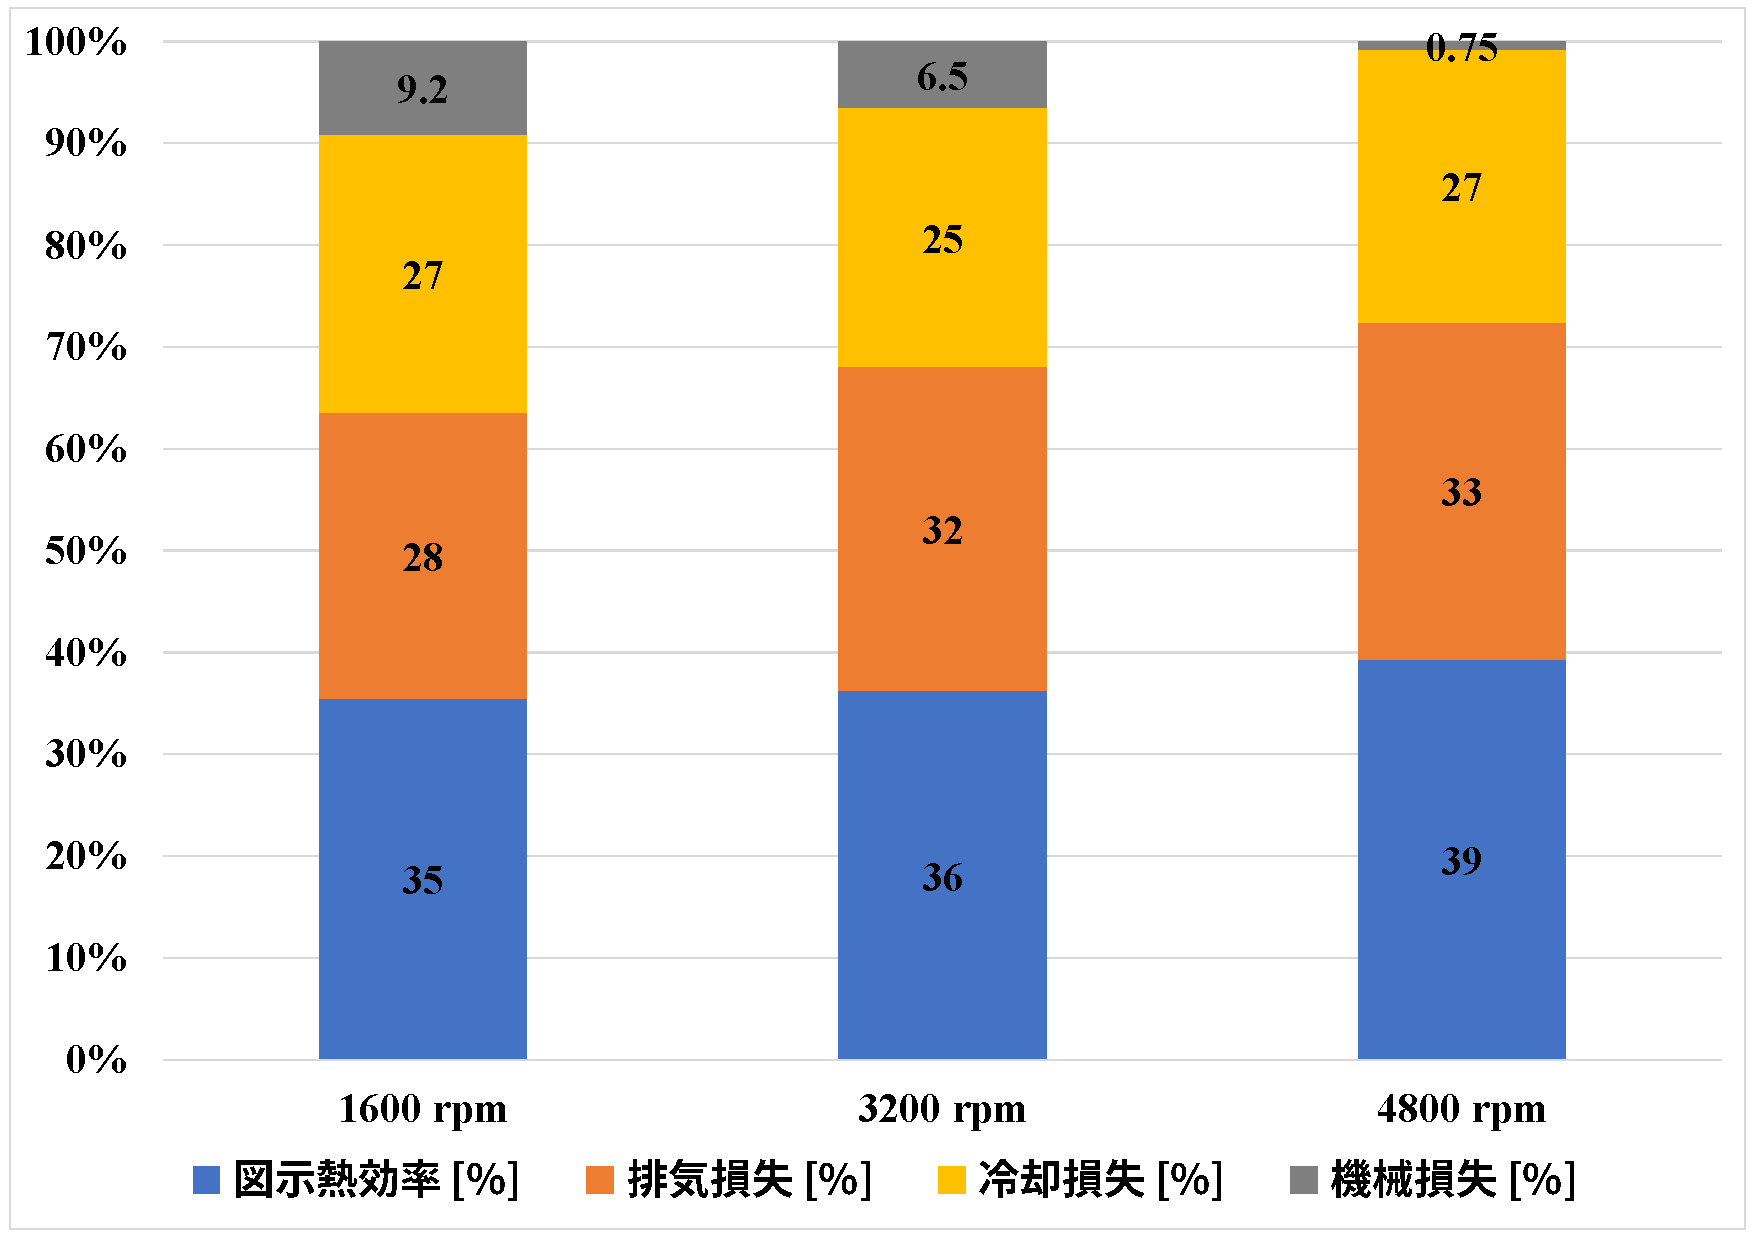
\includegraphics[width=.48\columnwidth]{img/zushi.pdf}
  \label{zushi}
  }
  \caption{熱勘定図}
  \end{center}
\end{figure}
\label{kanjou}

\clearpage

\mysection{考察}
実験結果より、冷却損失はほとんど一定であるが、排気損失がエンジンの回転数の上昇に伴ってやや増加する傾向にある。
$p$-$v$線図に関して、エンジンの回転数が4800\si{[rpm]}の際に、2$\rightarrow$3の過程において、
3における圧力が最も高く、最も直線的な形状であった。この過程は爆発的な燃焼が行われる。
表\ref{tb2}より、4800 \si{[rpm]}の際に、燃料全熱量の値が最も大きな値であったことから、
エンジンへの供給熱量が増加したためだと考えられる。また、圧力が最も高い値をとったため、
4800 \si{[rpm]} が最も熱効率が良いエンジン回転数であると考えられる。

今回実験に使用したエンジンの仕様から理論熱効率$\eta_{th}$を算出すると、式\eqref{eq1}のようになる。
\begin{equation}
  \eta_{th} = 1-\frac{1}{\varepsilon^{\kappa-1}}=1-\frac{1}{10.5^{(1.4-1)}}\fallingdotseq 0.61
  \label{eq1}
\end{equation}
つまり$\eta_{th}=\tsuyo{61\si{[\%]}}$である。


実験結果より、正味熱効率は28~30\%の値となるため、空気理論サイクルにおける理論熱効率に算出された熱(60\si{[\%]})の約半分が軸出力以外に使われたことを示している。
これらの熱は、エンジンの回転数の増加に伴い、エンジンで大きな音が生じたことや、冷却水の温度上昇、燃料消費率の上昇に伴う排気の増加(ガス交換による損失も含める)によって、
エンジン内の部品同士の摩擦による機械損失、冷却損失、排気損失に変換されたと考えられる。

また、図示熱効率はエンジンの回転数と図示出力に伴って増加する。冷却損失、排気損失は一定の
ため機械損失が減少する。しかし、実際は、エンジン内の部品の摩擦が生じるため、
機械損失がパラメータとなり、正味熱効率が減少する。よって、熱勘定図における図示熱効率と正味熱効率の偏差は、
機械損失の増加に起因すると考えられる。


これらから、\tsuyo{エンジンの高効率化}を図るために考えられることをいくつか提案する。
1つ目に\tsuyo{機械損失}を減少させるために、エンジンの熱で気化しない潤滑材を使用し、\tsuyo{摩擦を軽減する}、
2つ目に、\tsuyo{排気損失}を減少させるために、\tsuyo{燃料密度と低位発熱量がより小さい燃料}に変える、
3つ目に、\tsuyo{冷却損失}を減少させるために、\tsuyo{比熱が大きな流体を冷却に用いる}等が考えられる。

\mysection{感想}
熱機関のエネルギー効率を考える際に、理論値と実験値の考え方を区別して考えるという感覚が機械独特のものだと感じた。
理論熱効率は全てが理想的な状態と仮定した値であり、図示効率は実際に機械を動かしたものを理論に当てはめて、どんな\tsuyo{入力}があったか
を計算したもので理論と実験の中間的な値となり、正味熱効率は、機械によって実際に\tsuyo{出力}された値である。
実際に変換されているエネルギーを算出するために考慮すべき点が、電気系と比べて多く(冷却・排気・摩擦等)複雑だと感じた。
電気系は、電気そのものを得るまでに発生した損失を全て排除してから考えるから効率が高いのかもしれないと感じた。

\end{document}